\chapter{Rare Word Prediction}

In this chapter we present the LAMBADA dataset, which will be used throughout this thesis to evaluate our different models. We also discuss the rare word problem and examine several RNN regularization techniques.

\section{The LAMBADA dataset}
\label{sec:lambada}

This dataset was first introduced in \cite{paperno2016lambada} as a challenging test set specifically designed to probe the genuine language understanding of state-of-the-art NLP models. In the authors' words, \textit{``models' effectiveness at picking statistical generalizations from large corpora can lead to the illusion that they are reaching a deeper degree of understanding than they really are''}. Below we can find an example extracted from the dataset:

\begin{figure}[H]
	\begin{mdframed}[linewidth=1pt]
	\begin{quote} 		
		\textbf{Context:} \textit{``Why?'' ``I would have thought you'd find him rather dry,'' she said. ``I don’t know about that,'' said \underline{Gabriel}. ``He was a great craftsman,'' said Heather. ``That he was,'' said Flannery.} \par
		\textbf{Target sentence:} \textit{``And Polish, to boot,'' said $\rule{1.2cm}{0.15mm}$} . \par
		\textbf{Target word:} \textit{Gabriel}
	\end{quote}
	\end{mdframed}
	\caption{Example of a LAMBADA passage} \label{fig:lambadaPassage}
\end{figure}

As illustrated in \autoref{fig:lambadaPassage}, the dataset consists of narrative passages formed by a \textit{context paragraph} (with an average length of 4.6 sentences) and a \textit{target sentence}. The objective is to predict the last word of the target sentence (known as the \textit{target word}). In this way, LAMBADA casts the complex task of evaluating language understanding into the simple and general word prediction framework of language modeling.

\subsection{Construction Process}

LAMBADA was built using a large initial dataset, BookCorpus , which was then distilled into a difficult subset. The original dataset features 5325 unpublished novels (after duplicate removal) and 465 million words \cite{zhu2015aligning}. Novels were then randomly divided into equally-sized training and development+test partitions. Models tackling LAMBADA are intended to be trained on raw text from the training partition, which encompasses 2662 novels and more than 200 million words.

In order to obtain the LAMBADA passages, an automated filtering step was first applied to the development+test partition. Specifically, passages from the initial candidate set were discarded if the target word was given a probability $\geq 0.00175$ by any of the four different standard language models (both neural and count based) that were used in this stage of the process.

To make it into the final dataset, the remaining passages were then evaluated by human subjects in a three-step process:

\begin{enumerate}
	\item A human evaluator had to guess the target word correctly based on the whole passage (comprising the context and the target sentence).
	\item A second human evaluator had to also guess the target word correctly in the same conditions.
	\item Finally, ten human evaluators had to fail at guessing the target word having access to only the target sentence and 3 allowed attempts.
\end{enumerate}

Due to the specifics of this process, the passages that finally were selected have the property of not being guessable by just relying on local context and require broader understanding, probing the long range capabilities of language models. The final development and test sets that constitute LAMBADA consist of 4869 and 5153 passages, respectively. Additionally, a control set containing 5000 unfiltered passages was also constructed to allow for comparisons between standard language modeling scenarios and LAMBADA.

\subsection{Dataset Analysis}

The authors theorize that the inspection of the LAMBADA data suggests that, in order for the target word to be predictable in a broad context only (which is the case of LAMBADA by design), it must be strongly cued in the broader discourse. \autoref{fig:lambadaContext} compares the proportion of passages in the LAMBADA and control sets that include the target word in the context:

\begin{figure}[H]
	\centering
	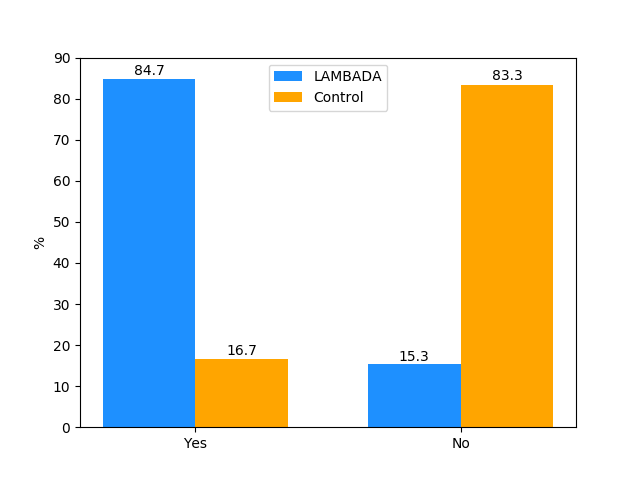
\includegraphics[scale=0.55]{lambadaContext}
	\captionof{figure}{Target word appears in passage.}
	\label{fig:lambadaContext}
\end{figure}

Indeed, in 84.7 \% of the LAMBADA items the target word (or its lemma, extracted with \texttt{nltk}'s WordNetLemmatizer) is mentioned in the context in the context, compared to the 15.3 \% for the control set. Furthermore, we can study the mention distance (understood as the number of words between the target word and its mention) distribution for LAMBADA. As illustrated in \autoref{fig:lambadaDistance}, 73 \% of the mentions are at a distance of more than 30 words (LAMBADA passages feature an average length of 75 words). This is specially important as many of the publicly available RNNLMs implementations are trained with TBPTT using $k_2$ somewhere between 20 and 35.
 
\begin{figure}[H]
	\centering
	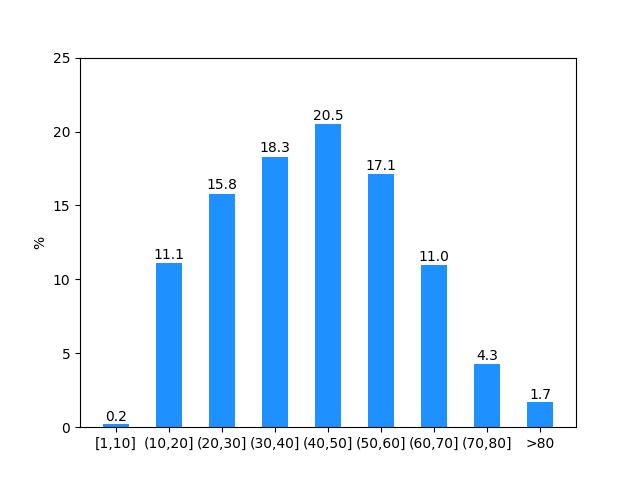
\includegraphics[scale=0.55]{lambadaDistance}
	\captionof{figure}{Target word appears in passage.}
	\label{fig:lambadaDistance}
\end{figure}

Moreover, it is also interesting to study the part of speech (PoS) tag distribution of the target words (also extracted with \texttt{nltk}'s default PoS tagger). As shown in \autoref{fig:lambadaPos}, proper nouns lead (48.1\%) followed by common nouns (37\%) and, far-off, verbs
(7.7\%). By comparing with control's PoS distribution, it is clear that proper nouns are over-represented in LAMBADA while the rest of the categories are downplayed.

\begin{figure}[H]
	\centering
	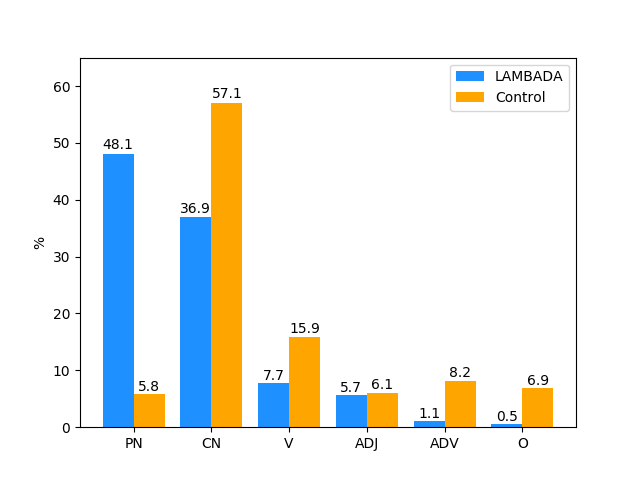
\includegraphics[scale=0.55]{lambadaPos}
	\captionof{figure}{Target words' PoS distribution (PN=proper noun, CN=common noun, V=verb, ADJ=adjective, ADV=adverb, O=other).}
	\label{fig:lambadaPos}
\end{figure}

\begin{figure}[H]
	\centering
	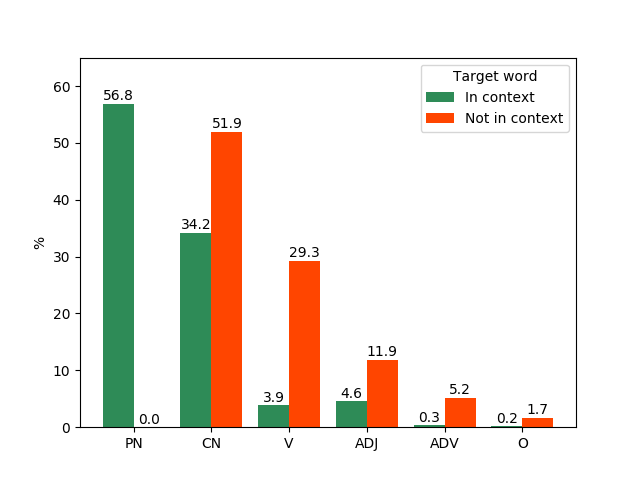
\includegraphics[scale=0.55]{lambadaPosAndContext}
	\captionof{figure}{LAMBADA target words' PoS distribution.}
	\label{fig:lambadaPosAndContext}
\end{figure}

The authors argue that the reason for this bias is the fact that proper nouns are favored by the specific setup. Namely, in many cases the context clearly demands a referential expression and the constraint of predicting a single word excludes other possibilities such as noun phrases with articles. This hypothesis seems to be confirmed by \autoref{fig:lambadaPosAndContext}, which shows the PoS distribution for LAMBADA split depending on whether the target word appears in the context. It can be seen that explicit mention in the preceding discourse context is critical for proper nouns (when the target word doesn't previously appear in the passage, none of them are proper nouns), while the other categories can often be guessed without having been explicitly introduced.

To sum up, we can conclude that LAMBADA does indeed put to the test language models' capabilities to exploit \textbf{long-range dependencies}. Besides, it is also important to note the bias towards proper nouns present in the dataset. Proper nouns are used to refer to unique entities (e.g. the name of a specific character in a book) and due to their very nature, they are \textbf{rare words} (when compared to the rest of the training corpus). We will describe this phenomena in detail in the next section.

\section{The Rare Word Problem}
\label{sec:problemRare}

As we saw in \autoref{chapter:nlm}, a common approach followed by recent neural language models is to use a softmax output layer where each of the dimensions corresponds to a word in a predefined vocabulary.

This approach has a fundamental problem, known as the \textit{rare word problem}. It is caused by some of the words in the vocabulary occurring much less frequently in the training set and thus, difficulting the learning of good representations for them and resulting in poor generalization performance. 

\begin{figure}[H]
	\centering
	\begin{subfigure}{.5\textwidth}
		\centering
		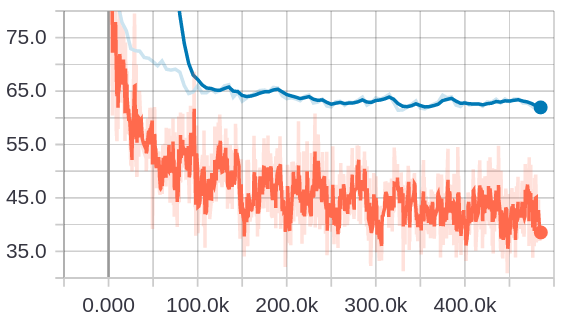
\includegraphics[scale=0.325]{perplexity_all}
		\caption{All words}
		\label{fig:perplexity_all}
	\end{subfigure}%
	\begin{subfigure}{.5\textwidth}
		\centering
		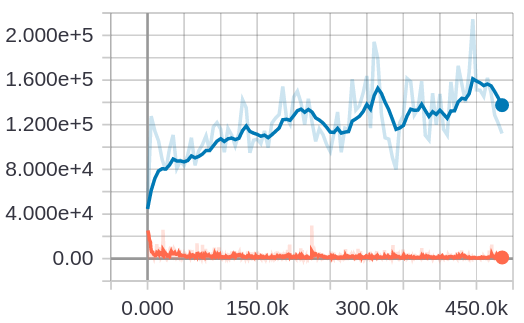
\includegraphics[scale=0.325]{perplexity_names}
		\caption{Only names}
		\label{fig:perplexity_names}
	\end{subfigure}
	\caption{Perplexity traces on LAMBADA (training trace is in orange and development, in blue).}
	\label{fig:perplexityRare}
\end{figure}

In \autoref{fig:perplexityRare} illustrates a real example of this problem. \autoref{fig:perplexity_all} shows traces of average word perplexity over training batches and the development set for a vanilla LSTM language model trained on the LAMBADA training partition (more details in \autoref{chapter:experiments}). If we now focus on just rare words (in this specific example, character names), we can see in \autoref{fig:perplexity_names} that the model is clearly overfitting on this subset of words. Intrinsically, rare words constitute a small fraction of the corpus and hence, their effect is averaged out when taking into account all words.

These results suggest that in general existing neural language models remain fundamentally lacking, failing to handle rare words.

\section{RNN Regularization}
\label{sec:rnnRegularization}

To end this chapter, we will describe in detail several recent efforts for effectively regularizing and avoiding overfitting in recurrent neural networks:

\subsection{Dropout}

Neural networks are very expressive models that can learn very complicated input-output mappings which may in turn lead to overfitting. Ensemble methods such as model averaging (where we average the outputs of several estimators that have been trained independently) are known to nearly always improve their single base estimators and have a regularization effect as the variance of the resulting model is reduced. However, the idea of averaging the outputs of many separately trained neural networks is prohibitively expensive. 

Dropout is an extremely effective and simple regularization technique introduced in \cite{srivastava14a}. It is implemented by only keeping a neuron active with some probability $p$ (a hyperparameter), or setting it to zero otherwise. If we consider a network with $n$ units, the application of dropout can generate $2^n$ different possible ``reduced'' networks (all of them sharing the same weights). In words of the authors, \textit{``training a neural network with dropout provides a way of approximately training a collection of $2^n$ thinned networks with extensive weight sharing, where actually each thinned network gets trained very rarely, if at all''}.

At test time, it is not feasible to explicitly average the predictions from exponentially many models. However, a very simple approximate averaging method is then used: no dropout is applied while testing and all weights are scaled by $p$ (same probability as used during training). This has the goal of ensuring that for any unit, the expected output (under the dropout distribution used in training time) is the same as the actual output at test time. Given a unit's output $y$, its expected value is $\mathbb{E}[y]=py+(1-p)0=py$.

In practice, we employ a variant known as \textbf{``inverted dropout''} where kept units are also scaled by $1/p$. This has the very appealing property of not requiring any additional operations during test time.

One of the first successful attempts at applying dropout for regularizing RNNs was described in \cite{zaremba2014recurrent}. The authors claim that dropout should only be applied to non-recurrent connections (namely, input and output units) by sampling a different dropout mask at each time step. Therefore it is ensured that information is only corrupted $L+1$ times (being $L$ the number of layers of the RNN), as exemplified in \autoref{fig:flowDropout}. In this way, the method can benefit from dropout regularization without sacrificing the valuable memorization ability of RNNs.

\begin{figure}[H]
	\centering
	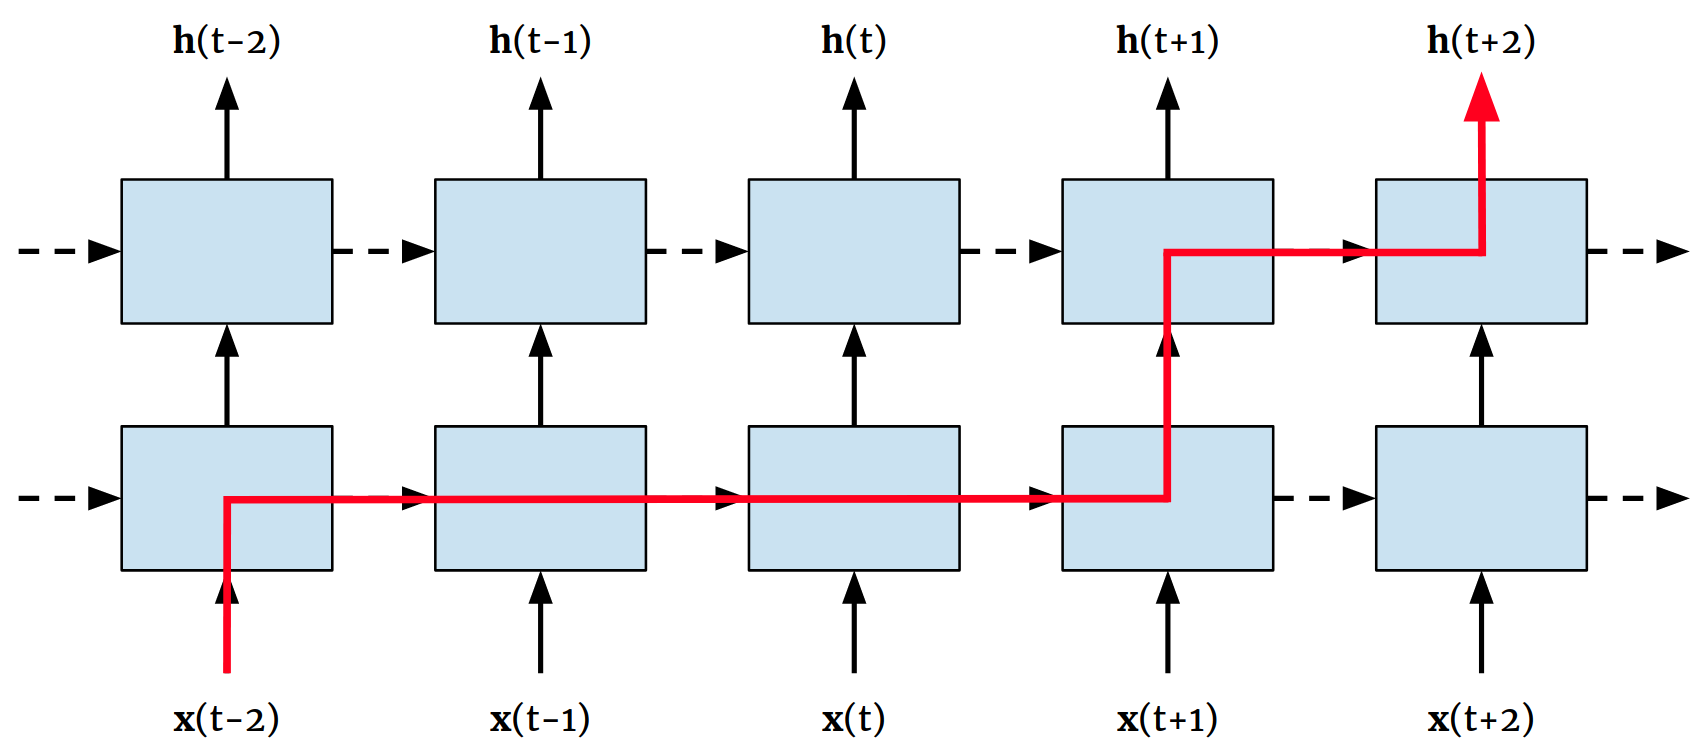
\includegraphics[scale=0.2]{flowDropout}
	\captionof{figure}{Example of information flow in a multilayer RNN with dropout (only applied at connections denoted with a solid arrow).}
	\label{fig:flowDropout}
\end{figure}

\subsection{Variational Dropout}

Following previous results at the intersection of Bayesian research and deep learning, \cite{gal2016theoretically} proposes a new dropout variant theoretically grounded on the results arisen from the application of approximate variational inference to probabilistic Bayesian RNNs. 

Given a training dataset consisting of the sequence of inputs $\mathbf{X}=\{\mathbf{x}(1),\\\cdots,\mathbf{x}(N)\}$ and outputs $\mathbf{Y}=\{\mathbf{y}(1),\cdots,\mathbf{y}(N)\}$, Bayesian parametric regression aims to infer the parameters $W$ of a function $\mathbf{y}=\mathbf{f}^W(\mathbf{x})$ (in our derivation, $\mathbf{f}^W(\cdot)$ is a neural network and $W$ are its weight matrices). Following the Bayesian methodology, we place a prior distribution $p(W)$ over the weights (often a standard multivariate Gaussian) and define a likelihood distribution $p(\mathbf{y} |\mathbf{x}, W)$ (usually assumed to be a softmax likelihood) and a posterior distribution $p(W | \mathbf{X}, \mathbf{Y})$ given the observed dataset.

For a new input point $\mathbf{x^*}$, an output can then be predicted as shown in \autoref{eq:post}. However this is not feasible in practice as the posterior is not tractable in general. 

\begin{equation} \label{eq:post}
\begin{gathered}
	p(W | \mathbf{X}, \mathbf{Y}) = \frac{ p(\mathbf{Y} | \mathbf{X}, W) p(W) }{ p( \mathbf{Y} ) } \\
	p(\mathbf{y^*} | \mathbf{x^*}, \mathbf{X}, \mathbf{Y}) = \int p(\mathbf{y^*} | \mathbf{x^*}, W) p(W | \mathbf{X}, \mathbf{Y}) dW
\end{gathered}
\end{equation}

To work around this problem, variational inference can be used to approximate the posterior with a variational distribution $q(W)$ and then
minimize the Kullback–Leibler (KL) divergence between the approximating distribution and the full posterior (\autoref{eq:varInference}). 

\begin{equation} \label{eq:varInference}
\begin{gathered}
	\mathcal{L}=\text{KL}(q(W)||p(W | \mathbf{X}, \mathbf{Y})) \propto - \int q(W) \log(p(\mathbf{Y} | \mathbf{X}, W))dW + \text{KL}(q(W)||p(W))\\
	= - \sum_{i=1}^{N} \int q(W) \log(p(\mathbf{y}(i) | \mathbf{f}^W(\mathbf{x}(i))))dW + \text{KL}(q(W)||p(W))
\end{gathered}
\end{equation}

Going now to the specifics of RNNs, we can further define each input point $\mathbf{x}$ to be a sequence $[\mathbf{x}(1),\cdots,\mathbf{x}(T)]$ of length $T$, the model output as $\mathbf{f_y}^W(\cdot)$ and the recurrent cell function as $\mathbf{f_h}^W(\cdot)$ (both of them with their respective weight matrices). Then the integral from \autoref{eq:varInference} can be rewritten as:

\begin{equation} \label{eq:approximation}
\begin{gathered}
	\int q(W) \log(p(\mathbf{y} | \mathbf{f_y}^W(\mathbf{h}(T))))dW \\ 
	= \int q(W) \log(p(\mathbf{y} | \mathbf{f_y}^W(\mathbf{f_h}^W(\mathbf{x}(T),\mathbf{h}(T-1)))))dW \\
	= \int q(W) \log(p(\mathbf{y} | \mathbf{f_y}^W(\mathbf{f_h}^W(\mathbf{x}(T),\mathbf{f_h}^W(\ldots\mathbf{f_h}^W(\mathbf{x}(1),\mathbf{h}(0)\ldots)))))dW \\
	\stackrel{*}{\approx} \log(p(\mathbf{y}| \mathbf{f_y}^{\hat{W}}(\mathbf{f_h}^{\hat{W}}(\mathbf{x}(T),\mathbf{f_h}^{\hat{W}}(\ldots\mathbf{f_h}^{\hat{W}}(\mathbf{x}(1),\mathbf{h}(0)\ldots))))) \, \text{with} \, \hat{W} \sim q(W)
\end{gathered}
\end{equation}

where $*$ means that the integral is approximated with Monte Carlo (MC) integration with a single sample.

Then the minimization objective can be formulated as:

\begin{equation} \label{eq:finalVarLoss}
\begin{gathered}
	\mathcal{L} \approx - \sum_{i=1}^{N} \log(p(\mathbf{y}(i) | \mathbf{f_y}^{\hat{W}}(\mathbf{f_h}^{\hat{W_i}}(\mathbf{x}(i,T),\mathbf{f_h}^{\hat{W_i}}(\ldots\mathbf{f_h}^{\hat{W_i}}(\mathbf{x}(i,1),\mathbf{h}(0)\ldots))))) \\ 
	+ \text{KL}(q(W)||p(W))
\end{gathered}
\end{equation}

It is important to note in \autoref{eq:finalVarLoss} that new weights are sampled for each point in the dataset. However, the weights are kept the same for all the time steps $t<T$ of every input sequence. Finally, the approximating distribution $q(W)$ is defined to factorize over the different weight matrices and their rows $\mathbf{w_k}$ as:

\begin{equation} \label{eq:approxPost}
	q(\mathbf{w_k})=p\mathcal{N}(\mathbf{m_k},\sigma^2\mathbf{I})+(1-p)\mathcal{N}(\mathbf{0},\sigma^2\mathbf{I})
\end{equation}

where $\mathbf{m_k}$ is a vector of variational parameters.

First we can see in \autoref{eq:approxPost} that sampling from $q(W)$ is identical to applying dropout on the weight matrices. Second, implementing the described approximate inference procedure is equivalent to performing dropout in RNNs with the same network units dropped at each time step, randomly dropping inputs, outputs, and recurrent connections. \autoref{fig:compareDropout} graphically illustrates the main differences of this method with respect to the one introduced in the previous section.

\begin{figure}[H]
	\centering
	\begin{subfigure}{.5\textwidth}
		\centering
		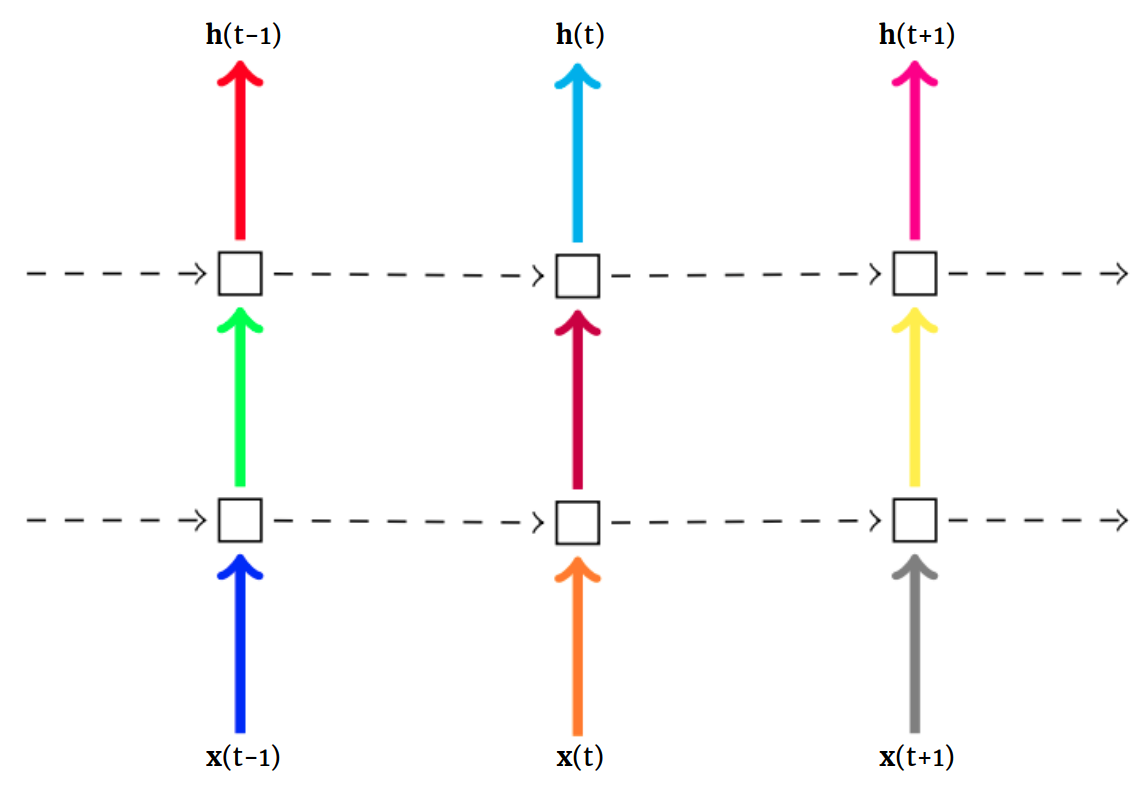
\includegraphics[scale=0.16]{dropout}
		\caption{``Naive''}
		\label{fig:dropout}
	\end{subfigure}%
	\begin{subfigure}{.5\textwidth}
		\centering
		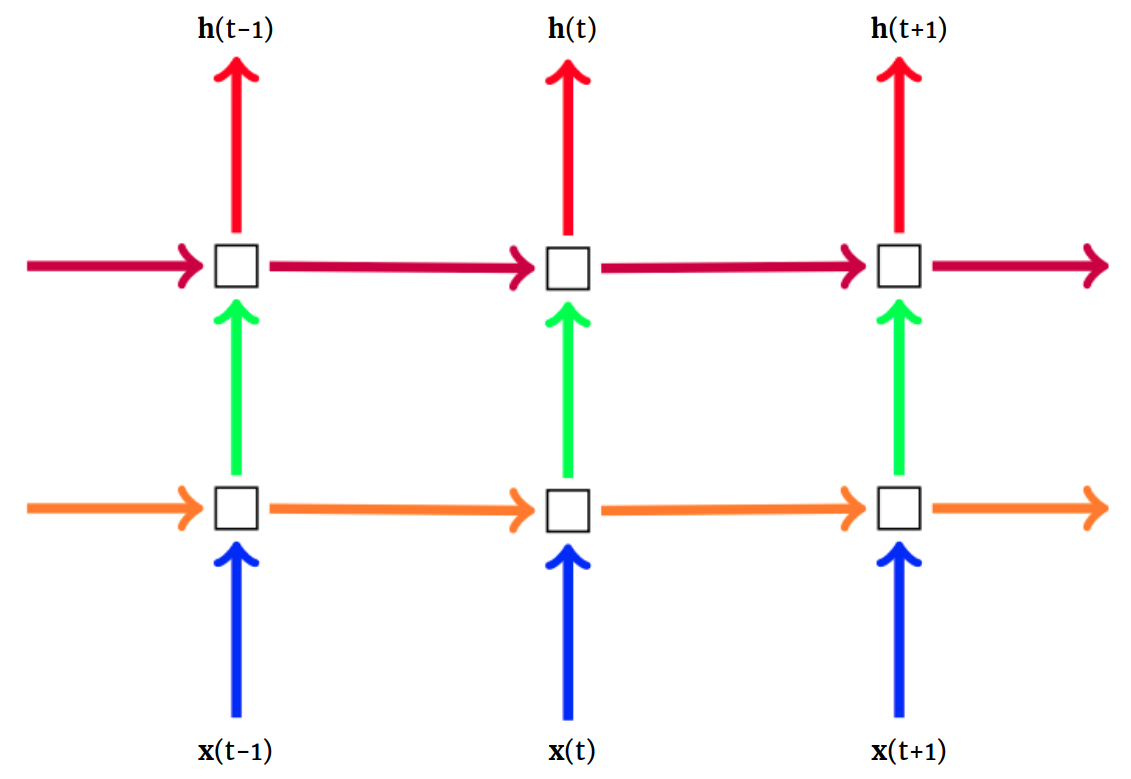
\includegraphics[scale=0.16]{varDropout}
		\caption{Variational}
		\label{fig:varDropout}
	\end{subfigure}
	\caption{Comparison of dropout techniques (only applied at connections denoted with a solid arrow, with different colors meaning different masks) \cite{gal2016theoretically}.}
	\label{fig:compareDropout}
\end{figure}

\subsection{Zoneout}

An alternative regularization method that only applies to the recurrent connections of an RNN was introduced in \cite{krueger2016zoneout}. Rather than setting a unit's activation to 0 with probability $1-p$ as in dropout, zoneout replaces the unit's activation with its value from the previous time step. We can see in \autoref{eq:zoneout} what is the formulation of zoneout for the LSTM cell:

\begin{equation} \label{eq:zoneout}
	\begin{gathered}
		\mathbf{c}(t) = \mathbf{d_c}(t)\odot\mathbf{c}(t-1) + (1-\mathbf{d_c}(t))\odot(\mathbf{f}(t) \odot \mathbf{c}(t-1) + \mathbf{i}(t) \odot \mathbf{\tilde{c}}(t)) \\
		\mathbf{h}(t) = \mathbf{d_h}(t)\odot\mathbf{h}(t-1) \\ 
		+ (1-\mathbf{d_h}(t))\odot (\mathbf{o}(t) \odot \tanh(\mathbf{f}(t) \odot \mathbf{c}(t-1) + \mathbf{i}(t) \odot \mathbf{\tilde{c}}(t)))
	\end{gathered}
\end{equation}

where $\mathbf{d_c}(t)$ and $\mathbf{d_h}(t)$ are Bernoulli random vectors.

It as argued by the authors that compared with dropout, zoneout is appealing because it preserves information flow forwards and backwards through the network. This in turn seems to help with the vanishing gradient problem, as shown by their experimental results.

\subsection{Weight Dropout}

The recent work described in \cite{merity2017regularizing} opts for applying DropConnect \cite{wan2013regularization} on the recurrent connections of a recurrent cell. For an LSTM, it is implemented by applying on the recurrent weight matrices ($U_f,U_i,U_o,U_f$ from \autoref{eq:lstmcell}) a Bernoulli mask  sampled before backward-forward pass. It is similar to variational dropout in the sense that the same mask is reused over multiple time steps. However by working directly on the weight matrices, ``weight dropout'' doesn't need to modify the formulation of the cell and is amenable to be used with highly optimized black box implementations.